\scanpage{67}\mspage{66}
% The raised inclusion and the long connecting stroke below the second row
% are reproduced with their formula labels; the labels occur only here.
\figure{
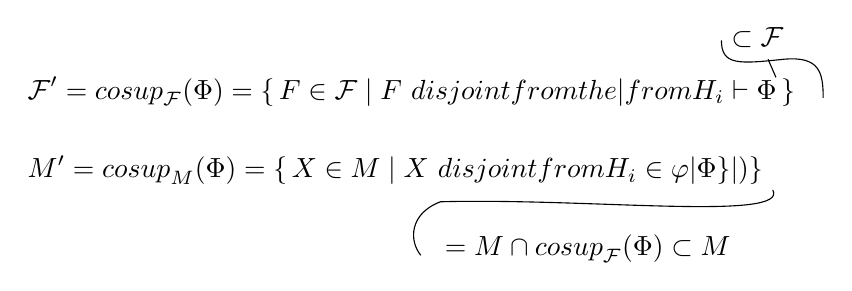
\begin{tikzpicture}[x=1cm,y=1cm,every node/.style={inner sep=0pt}]
  \node[anchor=west] (top) at (0,0) {$\displaystyle
    \mathcal F'=\operatorname{cosup}_{\mathcal F}(\Phi)
    =\{\,F\in\mathcal F\mid F\ \text{disjoint \unsure{from the|from} }H_i\vdash\Phi\,\}$};
  \node[anchor=south east] (addition) at ([xshift=-.15cm,yshift=.55cm]top.east)
    {$\inserted{\subset\mathcal F}$};
  \draw ([xshift=-.12cm,yshift=.1cm]addition.south west)
    .. controls ([xshift=-.12cm,yshift=-.22cm]addition.south west)
    and ([xshift=.1cm,yshift=-.2cm]addition.south west)
    .. ([yshift=-.14cm]addition.south east)
    .. controls ([xshift=.45cm,yshift=-.1cm]addition.south east)
    and ([xshift=.35cm,yshift=.25cm]top.east)
    .. ([xshift=.35cm,yshift=-.08cm]top.east);
  \draw ([xshift=-.2cm,yshift=-.14cm]addition.south east)
    -- ([xshift=-.25cm,yshift=.18cm]top.east);
  \node[anchor=west] (second) at (0,-1) {$\displaystyle
    M'=\operatorname{cosup}_{M}(\Phi)
    =\{\,X\in M\mid X\ \text{disjoint from }H_i\in
    \unsure{\varphi|\Phi}\unsure{\rbrace|)\rbrace}$};
  \node[anchor=west] (third) at (5.3,-2) {$\displaystyle
    \inserted{=M\cap\operatorname{cosup}_{\mathcal F}(\Phi)\subset M}$};
  \draw ([xshift=.12cm,yshift=-.25cm]second.east)
    .. controls ([xshift=.33cm,yshift=-.65cm]second.east)
    and ([xshift=-1.8cm,yshift=.65cm]third.east)
    .. ([xshift=-.05cm,yshift=.6cm]third.west)
    .. controls ([xshift=-.45cm,yshift=.45cm]third.west)
    and ([xshift=-.45cm,yshift=.1cm]third.west)
    .. ([xshift=-.3cm,yshift=-.08cm]third.west);
\end{tikzpicture}}

\deleted{Thus \unsure{we shall have|we have}, for $F\in\mathcal F$ setting $\mathcal F'=\operatorname{cosup}_{\mathcal F}$,}

\[
\begin{aligned}
&\deleted{\unsure{\phi|\Phi}}\qquad
\deleted{\mathcal F'=\operatorname{cosupp}_{\mathcal F}(\Phi),\quad M'=\mathcal F'\cap M,}\\[-2pt]
&\qquad\deleted{F\in\operatorname{cosup}_{\unsure{,|\mathcal F}}}
\qquad\qquad\deleted{=\operatorname{cosup}_{\deleted{\unsure{\mathcal F}}M}(\mathcal F)}
\end{aligned}
\]

Thus for $F\in\mathcal F$

% Slanted left marginal note, the brace display, and the right marginal
% note are one graphical group. Neither margin text is duplicated.
\figure{%
\begin{tikzpicture}[x=1cm,y=1cm,every node/.style={font=\small}]
\node[anchor=west] (brace) at (4.0,0) {$\displaystyle
\left\{\begin{aligned}
F\in\mathcal F'&\Longleftrightarrow\overline F\subset M'\\
M'&=.\mathcal F'\cap M
\end{aligned}\right.$};
\node[anchor=east,align=left,rotate=13] (leftnote) at (3.35,-.3)
  {Thus, $M'$ and $\mathcal F'$\\\unsure{determine|determine}\\\unsure{each other}};
\node[anchor=east] at (3.75,.26) {$\unsure{\longrightarrow}$};
\node[anchor=north west,align=left] (rightnote) at (11.0,1.0)
  {NB $\mathcal F',M'$\\are\\closed\\subsets of\\$\mathcal F,M$.};
\node[anchor=base west] (familylabel) at (10.3,-1.0) {$\mathcal F'$};
\node[anchor=base west] (stable) at (10.35,-1.51) {\uline{Stable under Sup.}};
\draw[line width=.7pt] (10.3,-1.1) -- (11.12,-1.1) -- (11.12,-.83);
\draw (8.75,-1.24) .. controls (9.5,-1.11) and (9.95,-1.1) .. (10.1,-1.4)
  .. controls (10.18,-1.66) and (12.5,-1.64) .. (13.8,-1.85);
\draw (10.43,-1.13) .. controls (10.05,-1.1) and (10.03,-1.7) .. (10.5,-1.71)
  .. controls (11.9,-1.75) and (13.4,-1.67) .. (14.1,-2.12);
\end{tikzpicture}%
}

Let on the other hand
\[
\begin{aligned}
\mathcal F''&=\operatorname{cosupp}_{\mathcal F}(\mathcal F')\overset{\text{def}}{=}\operatorname{supp}_{\mathcal F}(\Phi)\\
M''&=\operatorname{cosup}_{M}(\mathcal F')\overset{\text{def}}{=}\operatorname{supp}_{M}(\Phi)
\end{aligned}
\]

We have \unsure{seen|indeed|the|there} $\mathcal F''\supset\Phi$, $\mathcal F''$ stable under \unsure{Sup|Supp}, \deleted{contains $\Phi$} and under passage \unsure{:|to} a subfigure. Let $\deleted{\unsure{M}}\overline\Phi=\bigcup_{H_i\in\Phi}\overline H_i$, then
\[
\begin{aligned}
\operatorname{cosup}_{\mathcal F}(\Phi)&=\operatorname{cosup}_{\mathcal F}(M_{\overline\Phi})\\
\operatorname{cosup}_{\deleted{\unsure{\mathcal F}}M\unsure{..|:}}(\Phi)&=\{\,\deleted{\unsure{\varnothing|x}}X\in M\mid X\ \text{disjoint from }\unsure{\forall|\mathrm{every}}\ Y\in M_{\overline\Phi}\,\}
\end{aligned}
\]
thus we are \unsure{reduced|back} to constructions in $M$. \S

\uline{Saturated subset \inserted{$\mathcal F_0$} of} $\deleted{\unsure{M}}\mathcal F$ : equal to the cosupport of its cosupport ($\text{with respect to }\mathcal F$)\unsure{-|.} 

% Raised M_0 and its distinct oblique insertion leader.
\figure{%
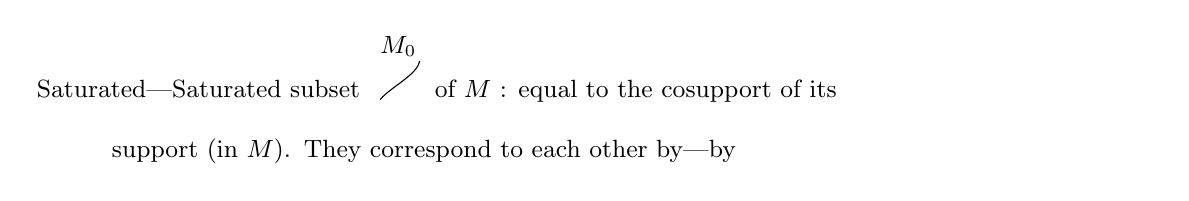
\begin{tikzpicture}[x=1cm,y=1cm,every node/.style={font=\small}]
\node[anchor=base east] at (3.4,0) {\unsure{Saturated|Saturated} subset};
\node[anchor=base] at (3.76,.55) {$\inserted{M_0}$};
\draw (4.03,.46) .. controls (4.01,.29) and (3.65,.12) .. (3.53,-.03);
\node[anchor=base west] at (4.1,0) {of $M$ : equal to the cosupport of its};
\node[anchor=north west,text width=13.2cm] at (0,-.4)
  {support (in $M$). They correspond \unsure{to each other} \unsure{by|\deleted{by}}};
\end{tikzpicture}%
}
\[
\begin{aligned}
M_0&=\mathcal F_0\cap M\\
\mathcal F_0&=\{\,F\in\mathcal F\mid\overline F\subset M_0\,\}
\end{aligned}
\]
